% Drawing 43/01-1 -- folder 43, batch 01, archive page 19 (PDF page 20).
% Transcription: schéma suivant, entre deux traits horizontaux et en partie entouré : $G(C)$ envoie une flèche vers $\prod G(\mathcal{O}_x)$ et une vers $G(K)$ ; ces deux groupes s'envoient sur $R^{0}_G$ ; de $R^{0}_G$ partent une flèche vers $J^{0}_G$ et une vers $\mathcal{D}iv^{0}_G$, qui aboutissent toutes deux, par des traits, à $H^1(X, G)^{0}$
% Kind: arrow diagram between two horizontal lines, partly enclosed. Method 2 (schematic redraw from the facsimile). Status: ok.
% Notes: G(C) -> prod G(O_x) and G(K); both -> R^0_G; R^0_G -> J^0_G and Div^0_G; both joined by strokes to H^1(X, G)^0. The two horizontal lines and the pencil strokes partly enclosing the left part are drawn; the small crosses on the arrows out of G(C) are left out.
% Coordinates: 1 unit = 1 mm = 1/100 of the crop width (bbox in page fractions: [0.05, 0.57, 0.75, 0.735]).
% Redrawn by Claude (claude-opus-5-5), issue #73, 2026-11-07; not checked by a human; not compiled (no TeX in the session).
% Rights: reproduces part of the work -- behind RENDER_TRANSCRIPTS, never published by itself.
\documentclass[tikz,border=3pt]{standalone}
\usepackage{amsmath,amssymb}
\usetikzlibrary{patterns,arrows.meta}
\tikzset{pencil/.style={black!45}, struck/.style={black!35}, mark/.style={circle,draw,inner sep=1.3pt}, pt/.style={circle,fill,inner sep=0.9pt}, opt/.style={circle,draw,fill=white,inner sep=1.1pt}}
\begin{document}
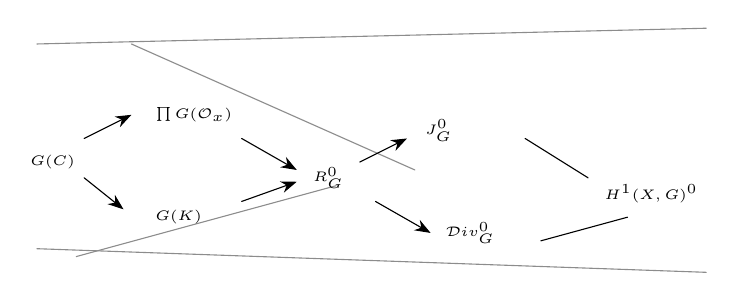
\begin{tikzpicture}[x=1mm,y=1mm,line cap=round,line join=round,font=\scriptsize]
\draw[pencil] (10,-4) -- (95,-2);
\draw[pencil] (10,-30) -- (95,-33);
\draw[pencil] (22,-4) -- (58,-20);
\draw[pencil] (15,-31) -- (48,-22);
\node[inner sep=1pt] at (12,-19) {\tiny $G(C)$};
\node[inner sep=1pt] at (30,-13) {\tiny $\prod G(\mathcal O_x)$};
\node[inner sep=1pt] at (28,-26) {\tiny $G(K)$};
\node[inner sep=1pt] at (47,-21) {\tiny $R^0_G$};
\node[inner sep=1pt] at (61,-15) {\tiny $J^0_G$};
\node[inner sep=1pt] at (65,-28) {\tiny $\mathcal{D}iv^0_G$};
\node[inner sep=1pt] at (88,-23) {\tiny $H^1(X,G)^0$};
\draw[-{Stealth[length=2mm]}] (16,-16) -- (22,-13);
\draw[-{Stealth[length=2mm]}] (16,-21) -- (21,-25);
\draw[-{Stealth[length=2mm]}] (36,-16) -- (43,-20);
\draw[-{Stealth[length=2mm]}] (36,-24) -- (43,-21.5);
\draw[-{Stealth[length=2mm]}] (51,-19) -- (57,-16);
\draw[-{Stealth[length=2mm]}] (53,-24) -- (60,-28);
\draw (72,-16) -- (80,-21);
\draw (74,-29) -- (85,-26);
\end{tikzpicture}
\end{document}
